\chapter{Implementation \label{sec:implementation}}

\begin{figure}[!htb]
    \centering
    \includegraphics[width=1\textwidth]{structurizr-1-veritest_solution_1.png}
    \caption{Software Architecture of Veritest}
    \label{fig:architecture}
\end{figure}

Figure \ref{fig:architecture} outlines the architecture implemented for VeriTest to implement a solver-based tool for finding incorrect optimizations,
referred by Lopes and Regehr \cite[p. 5]{CompilerOptimization}. 
VeriTest is available in online repository\footnote{\href{https://github.com/achmadafriza/veritest-dev}{https://github.com/achmadafriza/veritest-dev}}. 
The API documentation for VeriTest can be 
accessed through Postman\footnote{\href{https://documenter.getpostman.com/view/12004801/2sA35D64D8}{https://documenter.getpostman.com/view/12004801/2sA35D64D8}}.
There are several key design decisions needed to achieve the functional and 
non-functional requirements of this project (See Sec. \ref{sec:PossibleApproaches}), all of which are outlined in the following sections.

\section{Isabelle as Proof Engine}
\label{sec:ProofEngine}

We leverage Isabelle's automated tools -- Sledgehammer to find proofs; Nitpick and Quickcheck to find counterexamples --
to carry out the analysis for each of the optimization rules. This is possible due to the intermediate 
representation (IR) of GraalVM represented as an inductive datatype inside Isabelle \cite[Sec. 3]{ATVA21_GraalVM_IR_Semantics}. 
This encoding allows Isabelle to automatically translate the encoding into datatypes internal to Isabelle \cite{biendarra_ning_2024}.
The efficacy of this method is outlined in Section \ref{sec:results}.

Furthermore, as the inductive datatype acts as the grammar of Veriopt's DSL, erroneous syntax can be detected automatically by Isabelle.
This is due to the fact that the inductive datatype expects certain types to be present in order for the optimization to be syntactically correct.

\begin{align}
    &\text{\textbf{optimization} \emph{WrongMultiplication: \((x\ *\ 1)\ \longmapsto\ x\)}} \label{eq:MalformedRule} \\
    &\text{\textbf{optimization} \emph{CorrectMultiplication:} \((x\ *\) (\emph{ConstantExpr} (\emph{IntVal} \(b\ 1\)))) \(\longmapsto\ x\)} \label{eq:CorrectRule}
\end{align}

In (\ref{eq:MalformedRule}), we see that the optimization is intuitively correct. However, as \((x\ *\ 1)\) is translated into 
\emph{BinaryExpr BinMul x 1}, Isabelle expects the syntax to be in the form of \emph{BinaryExpr BinMul IRExpr IRExpr} 
\cite[Definition 1]{Term_Graph_Optimizations}. With type unification, we can infer that \(x\) is of type \emph{IRExpr}. However, \(1\) is 
internally encoded in Isabelle as an Isabelle word, not an IR expression \cite[Definition 2]{Term_Graph_Optimizations}. We can amend the 
optimization rule by defining it as (\ref{eq:CorrectRule}). As such, syntax errors can be detected.

\section{Mutual Exclusion}
\label{sec:MutualExclusion}

\begin{figure}[!htb]
    \begin{alignat}{3}
        \text{\textbf{optimization} } & \text{\emph{WrongOptimization}} & : \quad & \text{\emph{\(x~+~y~\longmapsto~x~-~y\)}} & \label{eq:WrongRule} \\
        & \text{\textbf{\emph{sorry}}} & & & \nonumber \\
        \text{\textbf{optimization} } & \text{\emph{ImpactedOptimization}} & : \quad & \text{\emph{\(x~*~1~\longmapsto~x\)}} & \label{eq:ImpactedRule} \\
        & \text{\textbf{\emph{nitpick}}} & & & \nonumber
    \end{alignat}

    \caption{Example of conflicting optimization rules}
    \label{fig:conflictingRules}
\end{figure}

As optimization rules are \emph{proposed} in VeriTest, the proposed optimization rule might be incorrect due to counterexamples. In Figure 
\ref{fig:conflictingRules}, we see that optimization rule (\ref{eq:WrongRule}) is obviously false due to arithmetic rules. But as we can omit 
proof for such optimization rules, by including the keyword \textbf{sorry}, this optimization rule is regarded as proven by Isabelle. This can 
impact the verification of optimization rule (\ref{eq:ImpactedRule}), falsifying the optimization rule, by the following reasoning:

\begin{align}
    z * 1\ &\longmapsto\ z,\ \text{(\ref{eq:ImpactedRule})} \\
    \nonumber \\
    Let\ z = (x + y) \\
    (x + y) * 1\ &\longmapsto\ (x + y) \\
    (x + y) * 1\ &\longmapsto\ (x + y)\ \longmapsto\ (x - y),\ \text{From (\ref{eq:WrongRule})} \\
    (x + y) * 1\ &\longmapsto\ (x - y) \\
    \nonumber \\
    Let\ x = 1,\ y = 1 \\
    (1 + 1) * 1\ &\longmapsto\ (1 - 1) \\
    2 * 1\ &\longmapsto\ 0 \\
    2\ &\longmapsto\ 0 \\
    &False
\end{align}

As such, it is critical for each of the \emph{proposed} optimization rule to be mutually exclusive with one another, only interacting with 
proven theories inside Veriopt's current theory base. This is aided by Isabelle's session framework \cite[Ch. 2]{isabelleSystem}, where 
each session only interacts with the imported theorems and lemmas inside of it, equivalent to Isabelle sessions defined for Isabelle/jEdit.
As such, optimization rules are analyzed by spawning a session for each of the rules and commands, depending on the current state of the 
analysis.

\section{Interfacing with Isabelle}
\label{sec:interface}

Regarding the non-functional requirement: 

\begin{quote}
    "Developers of GraalVM need to be able to integrate this easily into their test suite"
\end{quote}

While developer experience is important with concerns of developer workflow, the only concern for this project is to demonstrate the full 
capabilities of the analysis done inside VeriTest. Providing capabilities of a language server protocol (LSP) would be challenging, 
as the grammar for Veriopt's DSL is not formalized yet (See Chapter \ref{sec:results}). Thus, the extent of \emph{how} GraalVM would integrate 
VeriTest into their test suite is out of the scope of this project. As such, it is imperative that VeriTest provides a \emph{generic} interface 
towards analyzing optimization rules.

\begin{figure}[!htb]
    \begin{lstlisting}
        interface IsabelleProcessInterface extends Closeable:
            (BlockingQueue, LockCondition) open()
            TaskId submitTask(TaskType, args)
    \end{lstlisting}

    \caption{Pseudocode for Isabelle Process Interface}
    \label{fig:IsabelleProcessInterface}
\end{figure}

We utilize the Isabelle Client-Server interface to interact with Isabelle. Interacting with Isabelle Server can be done in several ways: 
through Isabelle Client, and through a TCP socket \cite[Ch. 4]{isabelleSystem}. For the purpose of VeriTest, we utilize Isabelle Client to 
simplify the implementation. Because of the possible alternatives, VeriTest abstracts the interactions through \mono{IsabelleProcessInterface}, 
as outlined in Figure \ref{fig:IsabelleProcessInterface}. Isabelle Process component outlined in Figure \ref{fig:architecture} implements 
this interface, and acts as a proxy for Isabelle Client.

\begin{figure}[!htb]
    \begin{lstlisting}
        interface IsabelleClient extends Closeable:
            Async<Task> startSession(request);
            Async<Task> stopSession(request);
            Async<Task> useTheory(request);
    \end{lstlisting}

    \caption{Pseudocode for Isabelle Client}
    \label{fig:IsabelleClientInterface}
\end{figure}

Furthermore, as any analysis done would only concern \emph{submitting} an optimization rule to analyze, VeriTest generalizes the interaction 
through \mono{IsabelleClient} interface, as illustrated in Figure \ref{fig:IsabelleClientInterface}. This interface generalizes any type of 
commands that would be invoked in Isabelle Server \cite[Sec. 4.4]{isabelleSystem}. This allows other components to focus on the implementation 
of the analysis, rather than worrying about how to interface with Isabelle.

\begin{figure}[!htb]
    \begin{lstlisting}
        abstract class AbstractIsabelleClient implements IsabelleClient:
            var Isabelle: IsabelleProcessInterface;
        
            Async<Task> startSession(request):
                return Isabelle.submitTask(START_SESSION, request)
                    then waitForCompletion()
                    then (TaskId) -> getResult(TaskId)
                    then switch (result):
                        case SuccessTask response -> return response;
                        case ErrorTask error -> throw error;
            
            ...
    \end{lstlisting}

    \caption{Pseudocode for Abstract Isabelle Client}
    \label{fig:AbstractIsabelleClient}
\end{figure}

As any interaction with Isabelle would involve the procedures of \mono{IsabelleClient}, we utilize a bridge pattern to abstract Isabelle's 
interaction, as seen in Abstract Isabelle Client in Figure \ref{fig:architecture}. The \mono{AbstractIsabelleClient}\footnote{\href{https://github.com/achmadafriza/veritest-dev/blob/master/src/main/java/com/veriopt/veritest/isabelle/AbstractIsabelleClient.java}{AbstractIsabelleClient.java} \& \href{https://github.com/achmadafriza/veritest-dev/blob/master/src/main/java/com/veriopt/veritest/isabelle/IsabelleProcess.java}{IsabelleProcess.java} extending \mono{AbstractIsabelleClient}} 
defines the procedures of how to interact with Isabelle, utilizing Isabelle Process, which can be seen in Figure \ref{fig:AbstractIsabelleClient}. 
\mono{stopSession()} and \mono{useTheory()} procedures use the same algorithm as \mono{startSession()} to define their interactions.
Note that \mono{then} keyword represent asynchronous function compositions. \mono{waitForCompletion()} waits for the 
asynchronous functions to complete. \mono{getResult()} is a procedure that handles demultiplexing tasks that allows for concurrent 
processes, which is elaborated in Section \ref{sec:ParallelExecution}.

It is worthy to consider that Isabelle responses in the form of \mono{Task} represents various types of responses from \mono{startSession()}, 
\mono{useTheory()}, \mono{stopSession()}, and even miscellaneous error messages from Isabelle \cite[Sec. 4.4]{isabelleSystem}. 
Each task would contain at least three fields: (1) their task identifier; (2) the type of message being sent, whether the corresponding task 
is finished or have errors; and (3) a list of messages from Isabelle. Through pattern matching Isabelle's messages, we can classify the result 
of the analysis, as elaborated on Section \ref{sec:generateAnalysis}. We parse 
Isabelle responses in the form of a string with a customized polymorphic deserializer called \mono{TaskDeserializer}\footnote{\href{https://github.com/achmadafriza/veritest-dev/blob/master/src/main/java/com/veriopt/veritest/isabelle/TaskDeserializer.java}{TaskDeserializer.java}}, 
which utilizes Jackson's \mono{ObjectMapper} \cite{fasterxml_objectmapper_nodate} -- that transforms a string into a abstract JSON tree -- 
with added functionality through Java Reflections API. This method of parsing is used extensively in Figure \ref{fig:IsabelleDaemon} that 
elaborates how to interface with Isabelle Client's subprocess.

Through this approach to interface with Isabelle, we provide modularity and extensibility for VeriTest, which would immensely assist 
GraalVM developers integration to their test suite and future work to be done.

\section{Parallel Execution}
\label{sec:ParallelExecution}

To support VeriTest's goal of providing fast analysis towards optimization rules, VeriTest utilizes concurrent processing by using asynchronous 
functions. The implementation of Isabelle Process and Abstract Isabelle Client utilizes a producer-consumer pattern, ensuring 
that interactions towards Isabelle Client would not be a bottleneck for other optimization rules.

\begin{figure}[!htb]
    \begin{lstlisting}
        class IsabelleProcess implements IsabelleProcessInterface:
            var processQueue : BlockingQueue;

            (BlockingQueue, LockCondition) open():
                startIsabelleSubprocess();
                queue := new BlockingQueue();

                var daemon := Daemon();
                daemon.processQueue := queue;
                daemon.notEmpty := new LockCondition();
                daemon.asyncQueue := new ReentrantLock();

                return (daemon.asyncQueue, daemon.notEmpty);
            
            synchronized TaskId submitTask(TaskType, args):
                writeToProcess(TaskType, args);
                
                var taskResponse := this.syncQueue.waitAndTake();

                return taskResponse.taskId;
            
            ...
    \end{lstlisting}

    \caption{Pseudocode for writing to process}
    \label{fig:IsabelleProcess}
\end{figure}

\begin{figure}[!htb]
    \begin{lstlisting}
        class Daemon:
            var processQueue : BlockingQueue;
            
            var notEmpty : LockCondition;
            var asyncQueue : BlockingQueue;
            
            void run():
                while process isAlive:
                    var string := readFromProcess();

                    var response := TaskDeserializer.parse(string);
                    switch (response):
                        case ImmediateTask -> this.processQueue.waitAndPut(response);
                        case AsyncTask -> {
                            this.asyncQueue.put(response);
                            signalAllCondition(this.notEmpty);
                        }
    \end{lstlisting}

    \caption{Pseudocode for reading from process}
    \label{fig:IsabelleDaemon}
\end{figure}

As Isabelle Client is a subprocess for VeriTest, we can split the input and output stream to efficiently process command invocations. 
The input stream would act as the producer towards the BlockingQueue, while the output stream would be continuously consumed by a separate 
thread -- as illustrated by Figure \ref{fig:IsabelleProcess} and \ref{fig:IsabelleDaemon}. This ensures that command invocations are only 
IO-bound by the input stream.

Isabelle Server has two types of responses that originate from command invocations: immediate responses and asynchronous responses 
\cite[Sec 4.2.6]{isabelleSystem}. Immediate responses denote the task identifier to differentiate between asynchronous responses, 
which is used by 
\mono{IsabelleProcess}\footnote{\href{https://github.com/achmadafriza/veritest-dev/blob/master/src/main/java/com/veriopt/veritest/isabelle/IsabelleProcessFacade.java}{IsabelleProcessFacade.java}}. 
Asynchronous responses denote the actual progress of the command invocation, 
identified by their task identifier. As we can see in Figure \ref{fig:IsabelleDaemon}, the types of responses are differentiated and sent 
to different queues.

\begin{figure}[!htb]
    \begin{lstlisting}
        class AbstractIsabelleClient implements IsabelleClient:
            var Isabelle: IsabelleProcessInterface;
            
            ...

            var asyncQueue, notEmpty := Isabelle.open()

            Async<Task> getResult(taskId):
                while true:
                    while asyncQueue is empty:
                        waitCondition(notEmpty);
                
                    if asyncQueue.peek().taskId == taskId:
                        return asyncQueue.take();
    \end{lstlisting}

    \caption{Pseudocode for getting asynchronous results}
    \label{fig:getResult}
\end{figure}

Asynchronous responses are consumed by the \mono{getResult()} method as illustrated by Figure \ref{fig:getResult}. Sufficient locking 
mechanisms without spinning the locks are done to ensure that concurrent processes accessing the same queue would not lead to starvation.
As the queue itself is a \mono{BlockingQueue}, and the purpose of the procedure is only to demultiplex the asynchronous responses, merely 
checking if the task has the correct identifier is enough to ensure mutual exclusion of concurrent processes.

\begin{figure}[!htb]
    \begin{lstlisting}
        Async<Void> allOfReturnOnSuccess(List<Async<Task>> futures):
            var futureResult := allOf(futures);

            for future in futures:
                future()
                    then (result) -> {
                        /* If the future is finished, and result is not failed, then terminate allOf() */
                        if future is successful && result.status != FAILED:
                            futureResult.complete();
                    }

            return futureResult;
    \end{lstlisting}

    \caption{Pseudocode for circuit-breaker asynchronous functions}
    \label{fig:circuitBreaker}
\end{figure}

Asynchronous functions are managed by a thread pool, separating IO bound processes into a different executor to ensure freedom from 
threadpool-induced deadlock. Furthermore, asynchronous functions implement a circuit-breaker pattern when a successful result is available 
from the function, which can be seen in Figure \ref{fig:circuitBreaker}. Through this, VeriTest is able to provide a \emph{comparatively} 
fast analysis for optimization rules with only Isabelle as a bottleneck (See chapter \ref{sec:results}).

\section{Generating the Analysis}
\label{sec:generateAnalysis}

VeriTest provides an API that encapsulates all the analysis that would be done towards the optimization rule 
in order to provide the functional requirements of VeriTest, and satisfy the non-functional requirement:

\begin{quote}
    "Developers of GraalVM can easily use this without understanding Isabelle."
\end{quote}

\begin{figure}[h]
    \centering
    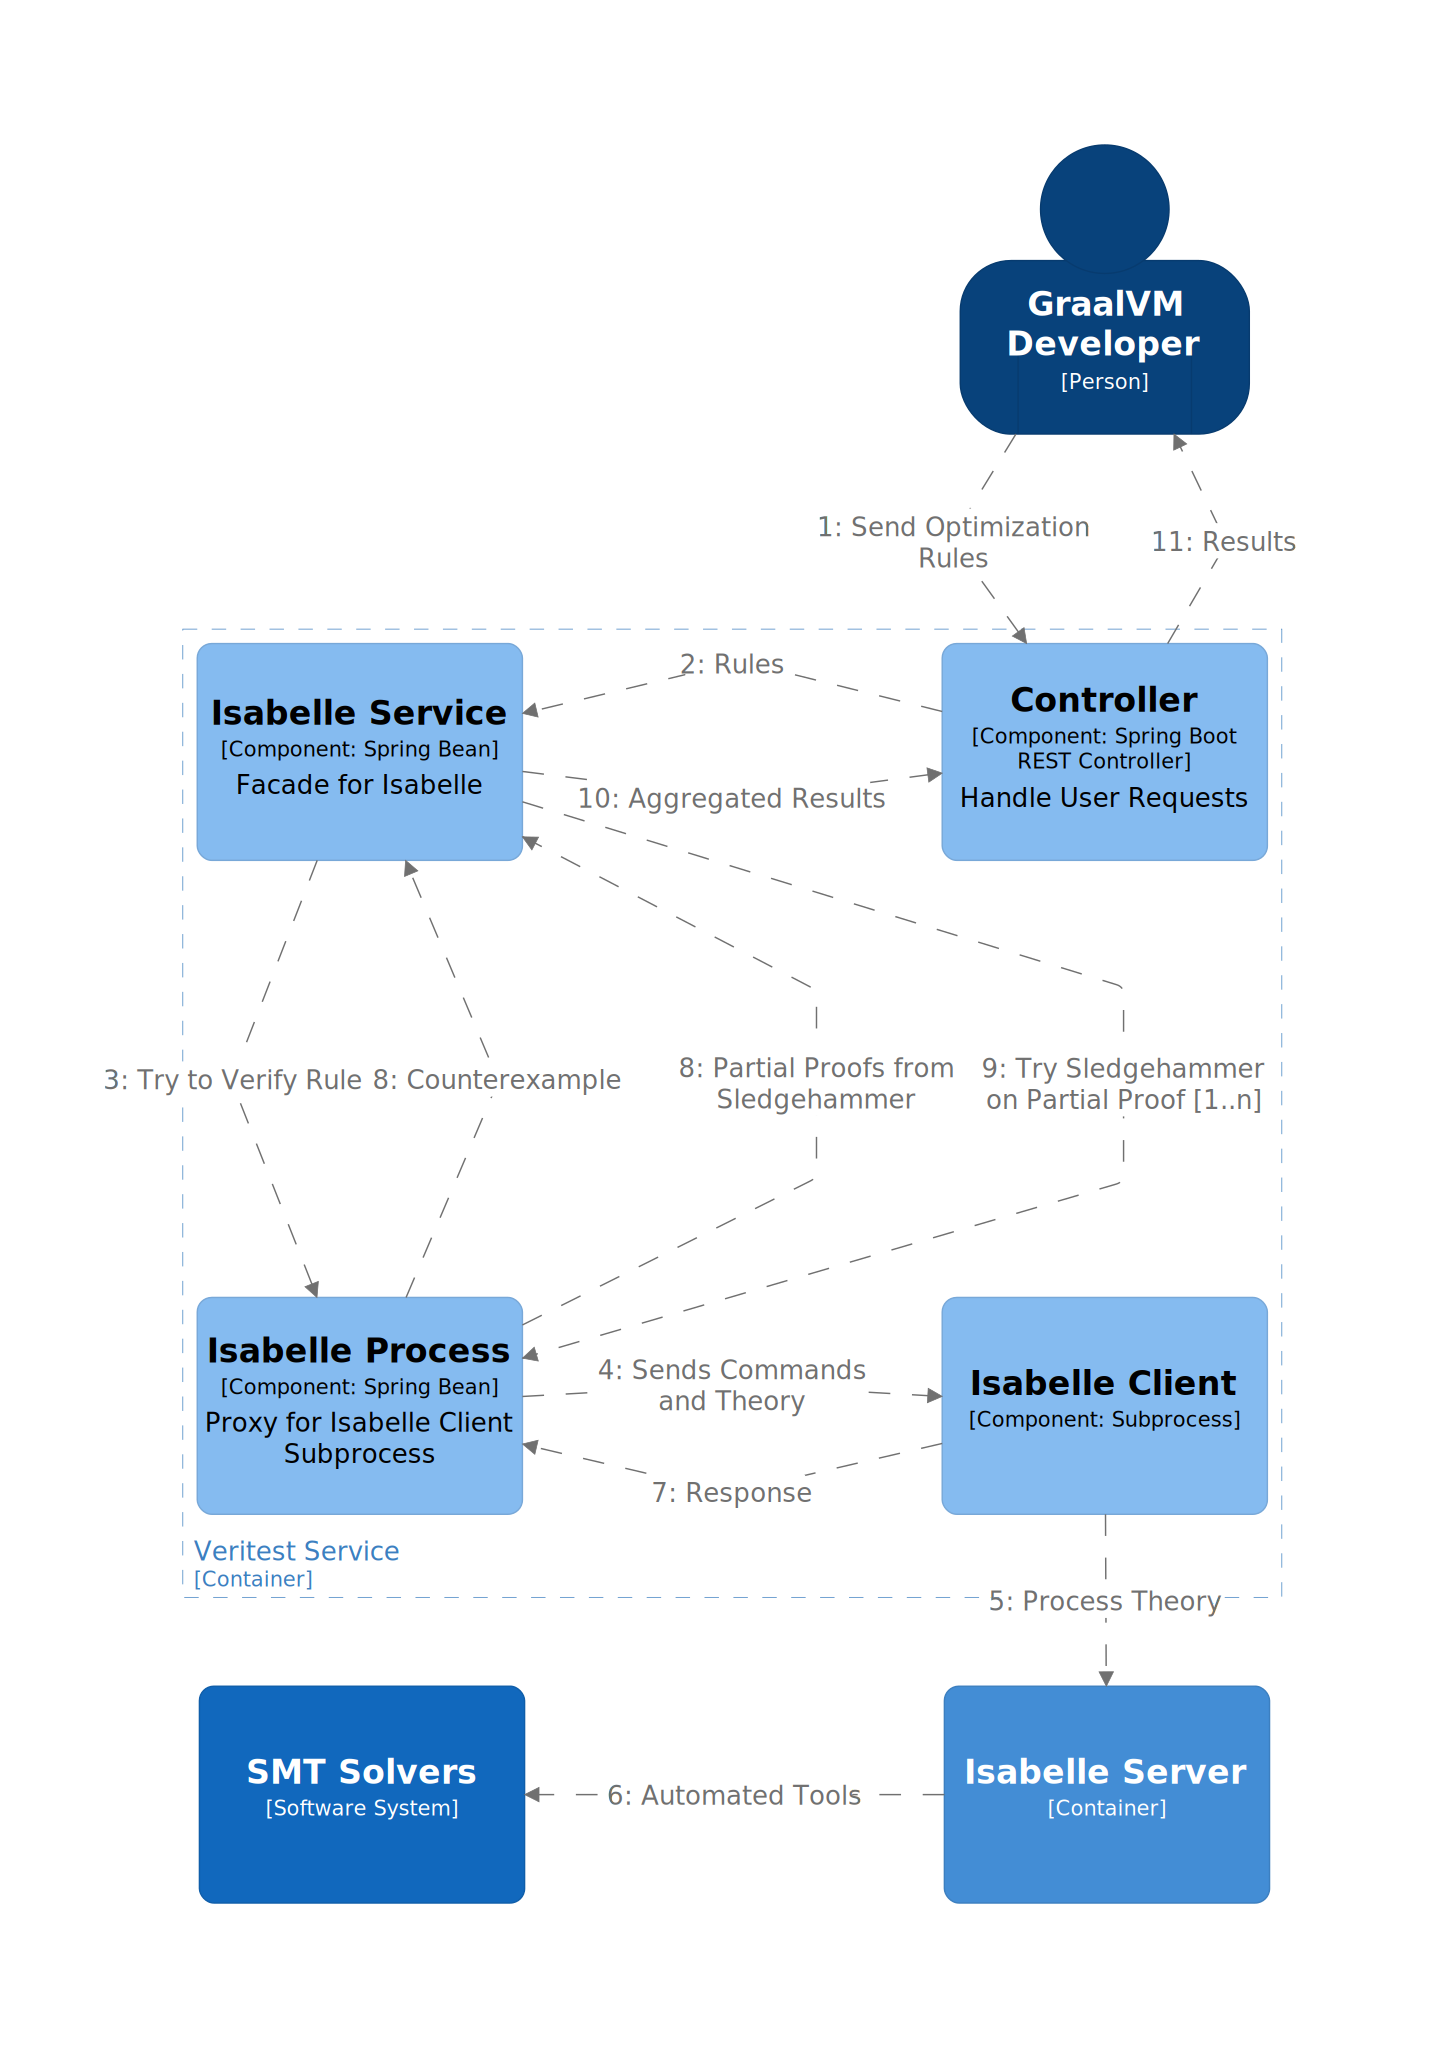
\includegraphics[width=0.9\textwidth]{structurizr-1-Dynamic-001.png}
    \caption{Sequence Diagram for VeriTest}
    \label{fig:sequenceDiagram}
\end{figure}

The analysis is done by invoking Isabelle's automated tools and pattern matching their response into their classification. 
The order of which the analysis is carried out can be seen in Figure \ref{fig:sequenceDiagram}. After significant 
evaluation and analysis, we extended their classification into multiple categories (See Figure \ref{fig:analysisClassification}).

\begin{figure}[!htb]
    \begin{tabular}{|L{0.95\textwidth}|}
          \hline
          \begin{enumerate}
                \item The optimization rule is false;
                
                    Quickcheck or Nitpick are able to find a counterexample.
            
                \item The optimization rule is automatically proven;
                
                    Based on the optimization rule, no proof obligation are necessary to proof that the optimization rule is true.  
                
                \item The optimization rule has no subgoals;
                
                    The optimization rule should be able to be automatically proven, but Isabelle classified the optimization as an error.
                    It is worthy to note that optimization rules that have no subgoals are specific to Isabelle2023, and 
                    should be amended by the next iteration of Isabelle.
                
                \item The optimization rule is proven;
                
                    Sledgehammer is able to prove the optimization rule.
                
                \item The optimization rule is malformed due to syntax errors;
                
                    The optimization rule does not follow the syntax of the DSL.

                \item The optimization rule is malformed due to type errors;
                
                    This means that the optimization rule provided has incompatible types.
            
                \item The optimization rule cannot be classified.
                      
                    VeriTest is unable to verify the optimization rule, due to the complexity of said rule.
          \end{enumerate} \\
          \hline
    \end{tabular}
    \caption{Extended classification of an optimization rule}
    \label{fig:analysisClassification}
\end{figure}

\subsection{Sledgehammer Invocations}

It is interesting to note that there are multiple invocations of Sledgehammer in order to find proofs towards an optimization rule. This is due 
to the fact that Sledgehammer can both return a partial proof towards an optimization rule due to the two proof obligations needed to prove an 
optimization rule, and return several proof options that can prove an optimization rule. A recursive algorithm is used in order to comprehensively 
prove an optimization rule, as illustrated by Figure \ref{fig:sledgehammerPseudocode}.

\begin{figure}[!htb]
    \begin{lstlisting}
        class IsabelleService:
            var Client: IsabelleClient;
            
            Async<Result> trySledgehammer(Theory):
                return generateTheory(SLEDGEHAMMER, Theory)
                    then Client.startSession(request)
                    then Client.useTheory(generated)
                    then recursiveSledgehammer(Theory, TaskResponse);
            
            Result recursiveSledgehammer(Theory, TaskResponse):
                /* Base Case: Errors returned from Isabelle */
                if TaskResponse contains errors:
                    return FAILED;
                
                /* Base Case: Found Proof */
                if TaskResponse contains "No Proof State" or "No Subgoal":
                    return (FOUND_PROOF, TaskResponse.proofs)
                
                var possibleProofs := filterProofs(TaskResponse);

                /* Base Case: Proof not found */
                if possibleProofs is empty:
                    return FAILED;
                
                var futures : List;
                for proof in possibleProofs:
                    var childRequest := generateChildRequest();
                    childRequest.proofs := TaskResponse.proofs + [proof];

                    futures.add(trySledgehammer(childRequest));
                
                allOfReturnOnSuccess(futures)
                    then waitForCompletion();

                var result := filterAnySuccessfulFuture(futures);

                return result;
    \end{lstlisting}

    \caption{Pseudocode for Sledgehammer recursive invocations}
    \label{fig:sledgehammerPseudocode}
\end{figure}

\subsection{Finding Counterexamples through Nitpick \& Quickcheck}

\begin{figure}[!htb]
    \begin{lstlisting}
        class IsabelleService:
            var Client: IsabelleClient;
            
            Async<Result> tryNitpick(Theory):
                return generateTheory(NITPICK, Theory);
                    then Client.startSession(request);
                    then Client.useTheory(generated);
                    then (Task) -> {
                        if Task contains error:
                            return FAILED;

                        if Task.messages contains counterexample:
                            return (FOUND_COUNTEREXAMPLE, counterexample);
                        else:
                            return FAILED;
                    };
            
            ...
    \end{lstlisting}

    \caption{Pseudocode for finding counterexamples}
    \label{fig:counterexamplePseudocode}
\end{figure}

Finding counterexamples are much more straightforward compared to Sledgehammer invocations. If any of the messages inside Isabelle's response 
contains a counterexample string, then a counterexample is found. This algorithm works with both Nitpick and Quickcheck invocations. As such, 
we can use an algorithm such as Figure \ref{fig:counterexamplePseudocode} to find incorrect optimization rules.

\subsection{Detecting Malformed Optimization Rules and Automatic Proof}

\begin{figure}[!htb]
    \centering
    \textbf{optimization} \emph{Auto: \((true~?~x~:~y)\ \longmapsto\ x\) .}

    \caption{Example of optimization rule that can automatically be verified}
    \label{fig:AutoExample}
\end{figure}

While we utilize Isabelle's automated tools to analyze our optimization rules, invoking a time consuming tool to detect malformed optimization rules 
is unnecessary. For some of the optimization rules (e.g., Fig. \ref{fig:AutoExample}), the rule is automatically verified by Isabelle due to it not 
having any necessary proof obligations to prove. As such, we can leverage this fact to invoke a quick and efficient automated tool in the form of a 
\textbf{dot} (.) that only does the reasoning internally. An algorithm such as Figure \ref{fig:malformedPseudocode} allows us to check for malformed 
optimization rules, type unification errors, and other types of errors.

\begin{figure}[!htb]
    \begin{lstlisting}
        class IsabelleService:
            var Client: IsabelleClient;
            
            Async<Result> tryAuto(Theory):
                return generateTheory(AUTO, Theory);
                    then Client.startSession(request);
                    then Client.useTheory(generated);
                    then (Task) -> {
                        if Task not contains error:
                            return FOUND_AUTO_PROOF;

                        if Task.messages contains "syntax error" or "undefined type":
                            return MALFORMED;
                        
                        if Task.messages contains "type unification error":
                            return TYPE_ERROR;

                        if Task.messages contains "no subgoal":
                            return NO_SUBGOAL;
                        
                        return (FAILED, Task.messages);
                    };
            
            ...
    \end{lstlisting}

    \caption{Pseudocode for finding malformed optimization rules}
    \label{fig:malformedPseudocode}
\end{figure}

\section{Dependencies and Containerization}
\label{sec:Containerization}

VeriTest is available as a containerized application\footnote{\href{https://hub.docker.com/repository/docker/achmadafriza/veritest}{https://hub.docker.com/repository/docker/achmadafriza/veritest}} 
ready for immediate use through Docker \cite{docker_inc_docker_2022}. All of the required dependencies of VeriTest are built through multiple build 
stages in order to reduce the time needed to build VeriTest through build caching. A critical component of VeriTest is utilizing Isabelle2023's Docker 
image to avoid rebuilding Isabelle from scratch \cite[Sec. 7.1]{isabelleSystem}.

Furthermore, VeriTest pre-builts all of the necessary lemmas and 
theorems from Veriopt's theory base in order to reduce the time needed to start a session for analyzing an optimization rule. It is important to note 
that Isabelle sessions needs to be built in the \emph{correct order}, beginning with Isabelle/HOL, dependencies of the Canonicalizations session from 
Veriopt's theory base, to the Canonicalizations session. The detail of the containerization can be seen in Appendix \ref{app:Containerization}.

\section{Supporting Tool}
\label{sec:Tool}

VeriTest also improves Veriopt's current extraction tool \cite[Sec. 7]{Term_Graph_Optimizations} by creating an extraction script capable of 
extracting source code annotations inside GraalVM's compiler and extracting Veriopt's existing optimization rules inside their theory base.
This extraction tool also serves as a test generation script for VeriTest, converting extracted optimization rules into JSON files. The details 
of this tool can be seen in Appendix \ref{app:supportTool}.